O objetivo da pesquisa é caracterizar dimensões afetivas negativas em perfis do twitter localizando pontos comuns entre usúarios portadores de afetividades negativas (stress, ansiedade e depressão) de mesmo nível. Esse tipo de processo se asemelha com a aprendizagem não supervisionada, logo, antes dessa etapa é necessário mapearmos atributos, sendo assim, é necessário a identificação de usúarios com dimensões afetivas negativas em primeiro momento.

Como observado, existem vários passos para conclusão desse projeto, abertamente estrutura de processamento contára com um processo de mineração e dois processos de inteligencia artificial afim de gerar dois modelos lógicos. O primeiro modelo responsavel por inferir valores da EADS em um perfil, e o segundo, de predizer, a partir de dados do perfil, a probabilidade de existir um determinado nível de afetividade utilizando dados do perfil.

 projeto em geral tem alguns outros pontos sociais envolvidos, sendo um deles captação de dados embasados através de profissionais, entretando, nosso objetivo inicial é fazer a máquina coletar e acertar as previsões com qualquer tipo de dado (mesmo que fornercido por pessoas não capacitadas), sendo assim, detalharemos o sistema em si (coleta de dados e aprendizagem de maquina) e as metodologias utilizadas para desenvolve-lo.

Pode-se observar na Figura \ref{fig:tecnologias}, o sistema é divido em dois núcleos, o Dumont responsável por minerar e gerar toda a base de dados, e o 14BIS que será responsavel pelas Inteligencias Artificias.

\begin{figure}
    \centering
    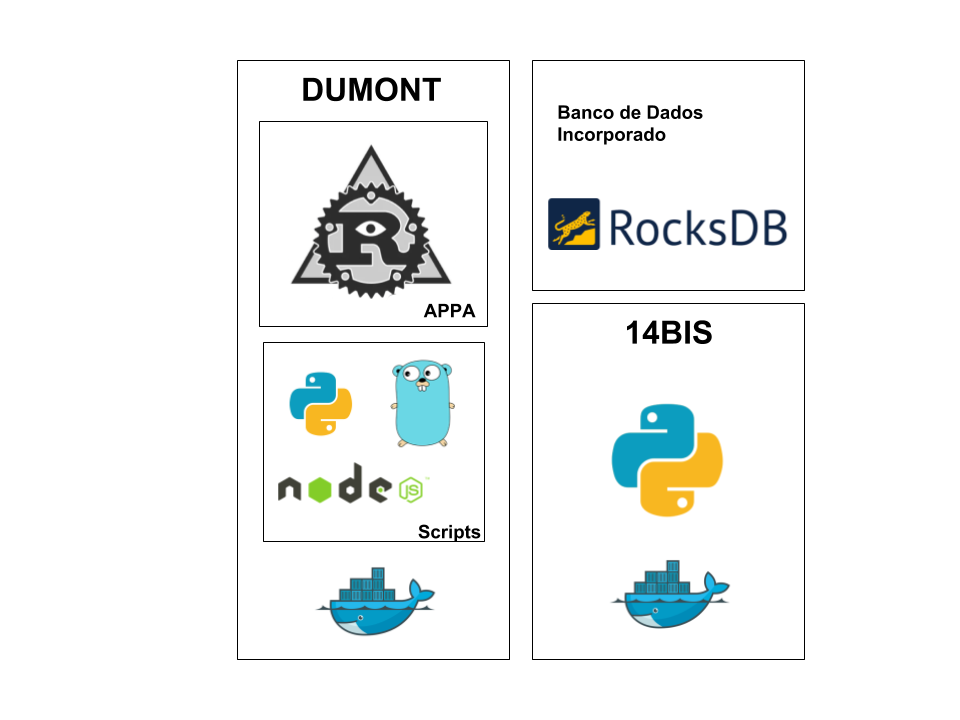
\includegraphics[width=1\textwidth]{imagens/tecnologias.png}
    \caption{Desenho apresentando os núcleos do projeto}
    \label{fig:tecnologias}
\end{figure}

Existem basicamente 5 técnologias que estão sendo utilizadas nesse projeto:
\begin{itemize}
 \item Python: É a linguagem atual mais utilizada no mundo de Aprendizado de Máquina, sua simplicidade ja á torna simples de usar, porém, a quantidade de materiais, bibliotecas e artigos sobre PLN e Aprendizado de Máquina á tornam a principal linguagem nesse projeto.
 \item Node/Javascript: Node é o interpretador que permite com que seja possivel executar o Javascript (linguagem originalmente de navegar no servidor). A linguagem tem um grande ganho com integrações e será utilizada para consumir recursos vindos de APIs.
 \item Go: Linguagem fortemente e estaticamente tipada, que fornecesse um poder de processamento equivalente a da linguagem C, entretando, muito mais simples de escrever e manter código, será utilizado para scripts onde serão necessário processamento de muitos dados.
 \item MongoDB: O Mongo é um banco não relacionado, em resumo, um grande banco de documentos indexados por atributos especificos, fornece um grande poder de leitura alem do fato de não ser prezo a estruturas pré-definidas como banco relacionais (isso facilita para que sejam inseridos novos dados futuramente sem grandes custos).
 \item Docker: Docker é uma ferramenta para infra-estrutura, será utilizado para rodar a aplicação em containers e facilitar o \textit{deploy}\footnote{Vindo do termo em inglês "lançar" é utilizado para o ato de colocar uma aplicação em ambiente de produção}.
\end{itemize}

Existirá uma sessão explicando todos os conceitos utilizados na mineração, assim como cada ferramenta usada em seu processo. Alem disso, será detalhada a parte  de Inteligencia Artificial, logo, nessa introdução os casos de uso serão tratados de forma sucinta. Se observar a Figura \ref{fig:tcc_caso_de_uso}, notara que o Dumont ira utilizar da API do twitter para coletar dados públicos, posteriormente esses dados serão processados e mutacionados a fim de gerar uma base de dados, por final essa base dados será salva em um banco de dados.

\begin{figure}
    \centering
    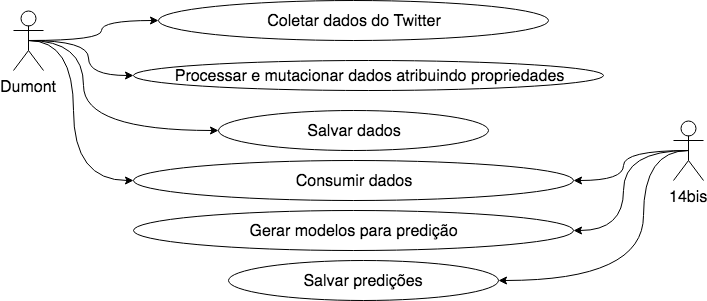
\includegraphics[width=.6\textwidth]{imagens/tcc_caso_de_uso.png}
    \caption{Diagrama de caso de uso do sistema}
    \label{fig:tcc_caso_de_uso}
\end{figure}

Para melhor entendimento a documentação será dividida em núcleos teóricos e práticos. Primeiramente será dado toda a descrição teórica sobre a escolha de atributos, e funcionamento das ferramentas que serão utilizadas no processo. Em seguida será detalhado os núcleos mais práticos como a coleta e mineração, onde alem de explicar como rodar o Dumont, tambem serão explicados como e por que foram construidas essas partes do sistema. Como ja dito, a primeira etapa se consiste em entender alguns dos atributos utilizados aqui.

\section{Engenharia de Atributos}
A escolha dos atributos, também intitulada popularmente como \textit{feature engineering}, é o ato mais importante durante a mineração de dados, por que é através desses atributos que as maquinas irão aprender. É válido destacar que essa sessão serve apenas para introduzir a razão dos atributos, seu detalhamento será dado durante a sua implementação.

O primeiro atributo relevante aqui é o sentimento. Já que será abordado dimensões afetivas negativas, o sentimento expressado por uma frase tem um grande impacto como atributo. Entretanto, o sentido em uma frase pode ser mais fácil de ser extraído em textos concisos, ou seja, normalizar os textos é necessário.

Um dos atributos utilizados aqui será o texto normalizado, para isso será utilizado o \textit{spacy}, uma biblioteca Python para remover palavras que oferecem apenas ruídos ao resultado. Além disso, também será tirada a arvore sintática, para que seja possível estabelecer padrões de discurso na IA, ou então, reconhecer certas palavras presentes em demais analises.

Uma vez observado os nossos atributos, seria necessário erguer um sistema capaz de realizar tarefas e persistir esses dados em algum banco de dados. Porém, será utilizado nessa pesquisa uma ferramenta para gerenciar tais tarefas.

\subsection{Git e Github}
O Git é uma ferramenta de versionamento de código, ou seja, uma ferramenta utilizada para que toda a alteração que alguém fizer em um código tenha a possibilidade de ser marcada, assim criando uma arvore das modificações e dando ao usuário a possibilidade de navegar entre suas alterações. A ferramenta foi criada por Linus Torvalds durante a criação de Linux, para que fosse possível manter um histórico seguro do desenvolvimento do sistema operacional. Entretanto, o Git é unicamente uma ferramenta de terminal, com o desenvolvimento da internet e os recursos gráficos sendo cada vez mais utilizados para representações, juntamente com a necessidade de algo mais acessível, nasceram varias interfaces para a ferramenta, uma delas e também a maior, o GitHub ganhou tração e é hoje uma das maiores plataformas de código aberta do mundo e recentemente foi adquirida pela Microsoft\footnote{\url{https://g1.globo.com/economia/tecnologia/noticia/microsoft-compra-github-por-us-75-bilhoes.ghtml}}.

É importante saber sobre Git nos dias de hoje, se quiser descobrir mais é possível achar todo o necessário em um livro\footnote{\url{https://git-scm.com/book/en/v2}} fornecido pela própria mantenedora da ferramenta. No caso desse trabalho é possível simplesmente baixar o código pelo Github. Para isso, vamos entender a interface do GitHub.

Se observar a figura \ref{fig:git_init}, pode-se notar um cabeçalho com alguns menus, logo abaixo o nome da organização getdumont seguida pelo nome do repositório\footnote{Repositório é o nome dado ao local onde ficará armazenado todo o código de um determinado projeto}. Então pode-se notar 5 abas, que nesse momento são irrelevantes, seguindo encontra-se alguns dados como descrição, algumas estatísticas e por fim o botão verde \textit{Clone or Download}, aqui pode-se baixar o código clicando no botão e em seguida clicando em \textit{Download ZIP}. Além disso, logo abaixo é possível ver uma tabela com a estrutura do projeto, essa estrutura é navegável pelo browser, assim qualquer arquivo citado durante essa documentação pode ser acessado sem necessidade do código na maquina.

\begin{figure}
    \centering
    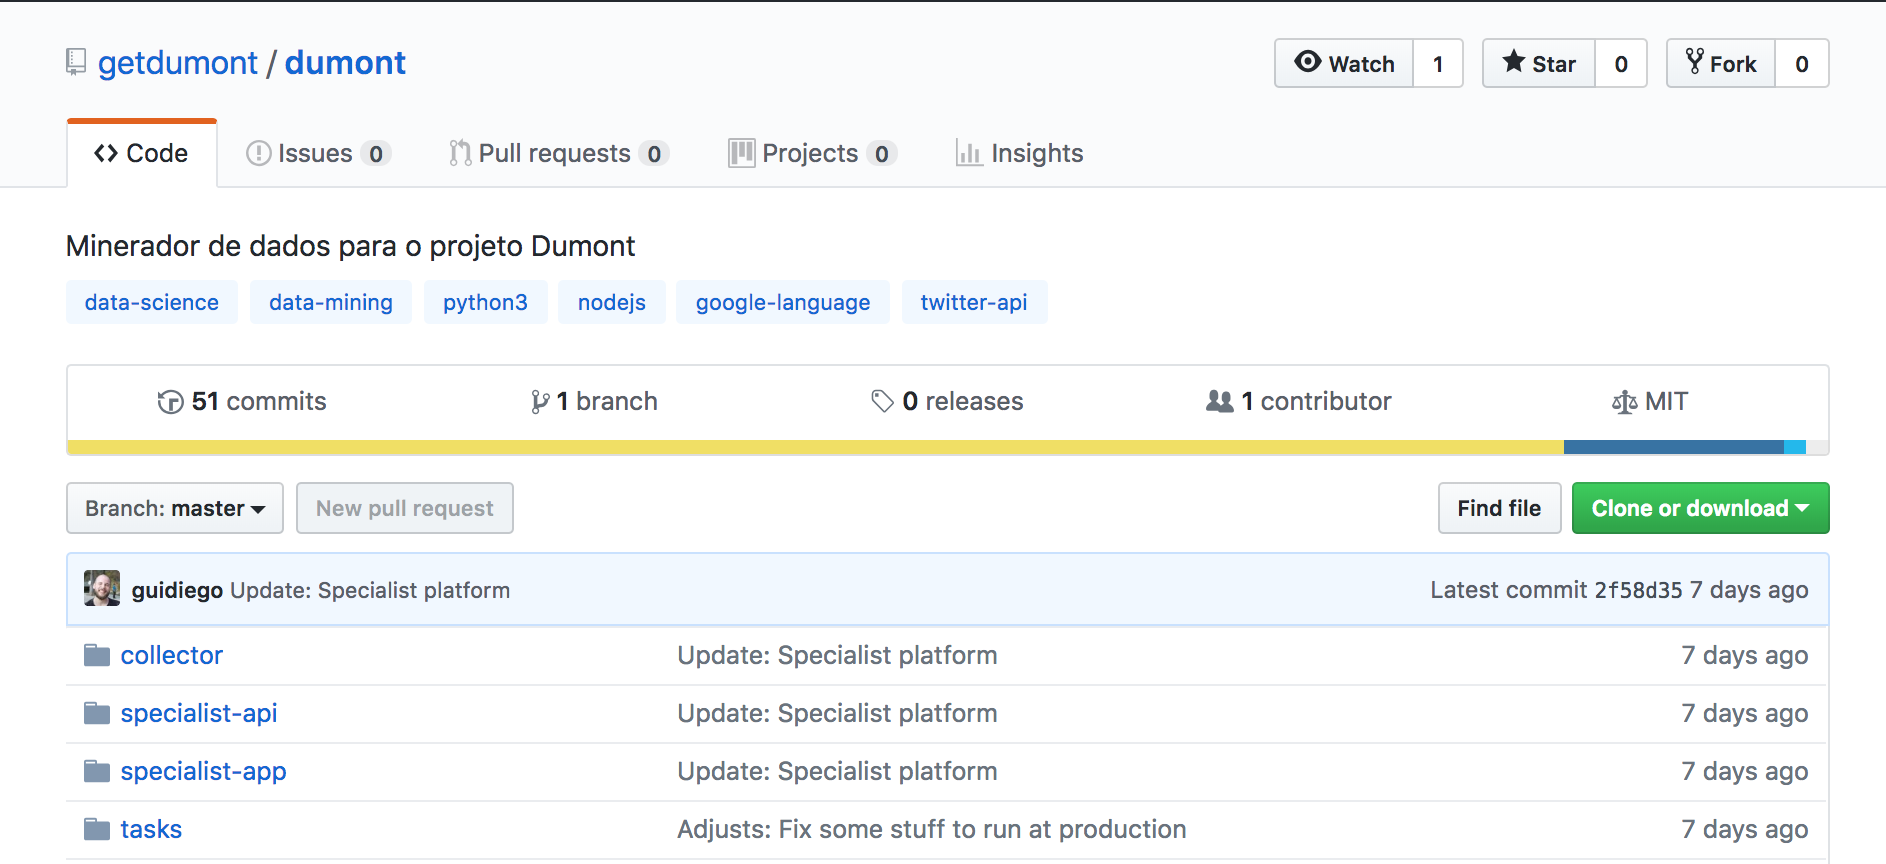
\includegraphics[width=.8\textwidth]{imagens/git_init.png}
    \caption{Imagem demonstrando a interface inicial do git}
    \label{fig:git_init}
\end{figure}

Já na figura \label{fig:git_file}, pode-se observar um exemplo do que foi dito anteriormente. Aqui uma demonstração de como fica um dos arquivos do projeto aberto no navegador. As 2 coisas mais importantes a serem notadas aqui é o caminho do arquivo \textit{dumont/collector/index.js} e as linhas que são mostradas no arquivo. Será utilizado destes recursos durante a documentação para exemplificar e apontar códigos.

\begin{figure}
    \centering
    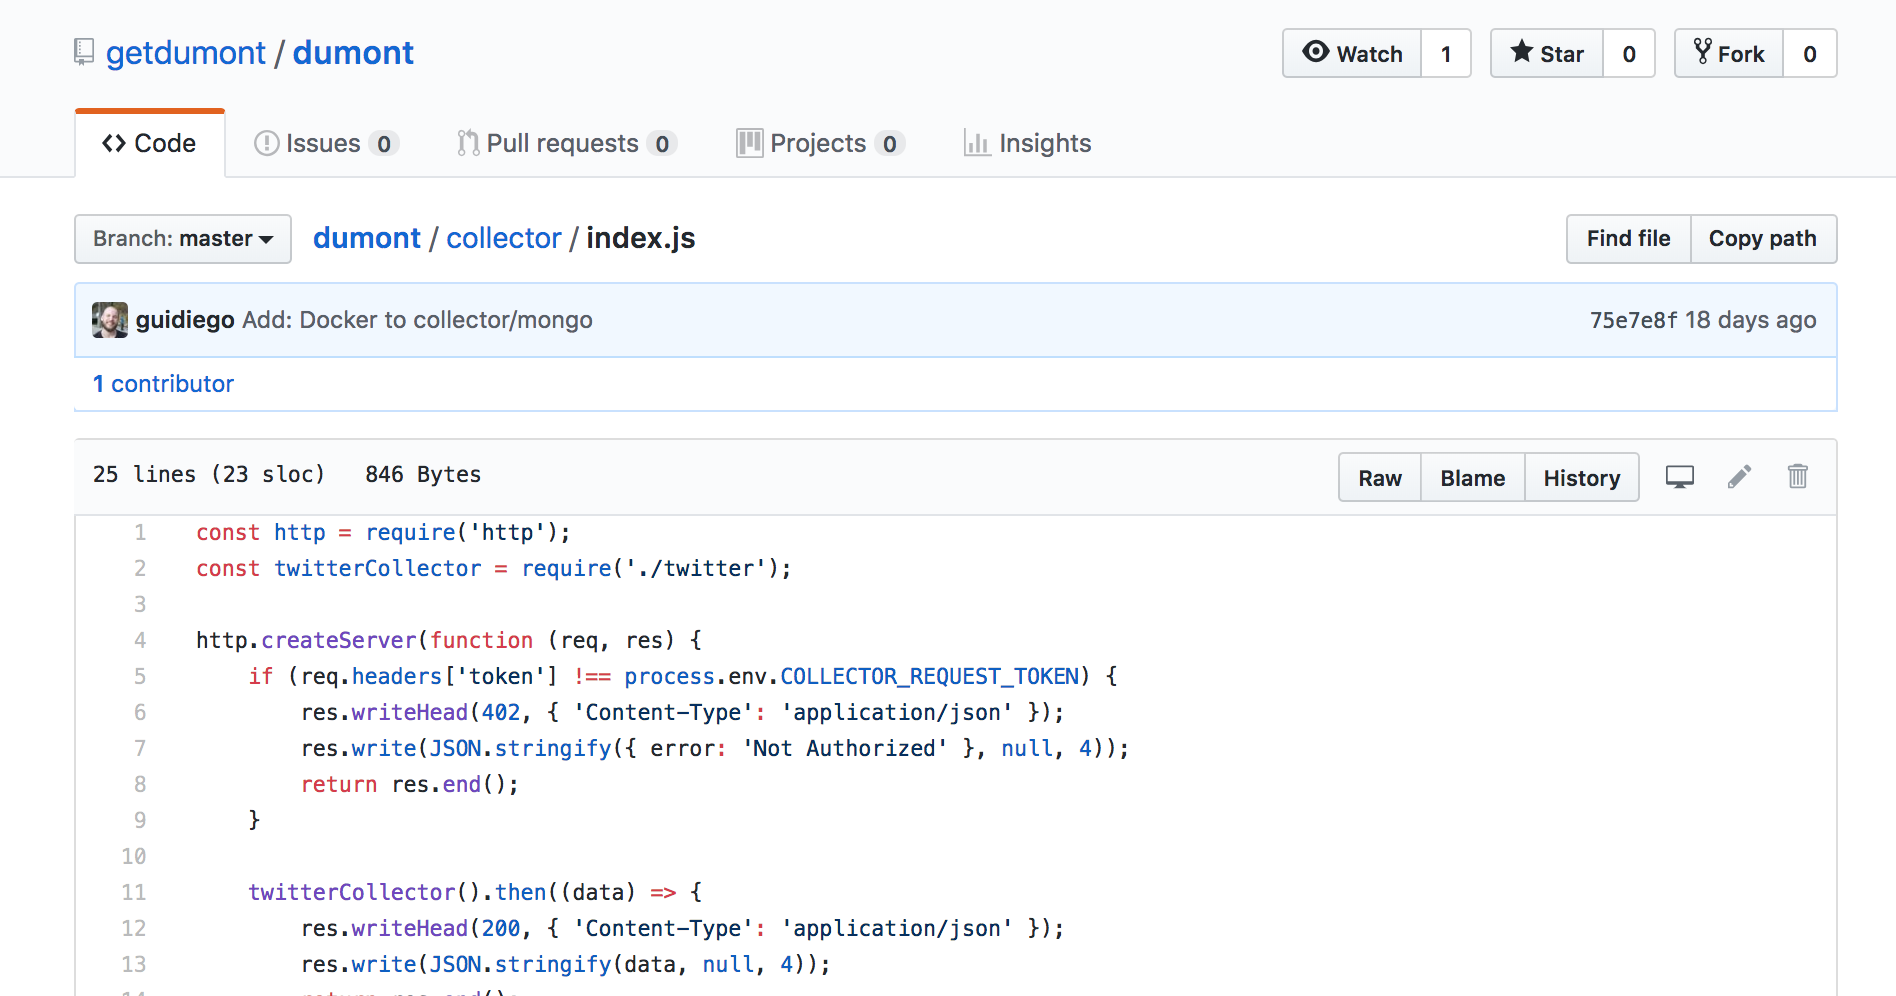
\includegraphics[width=.8\textwidth]{imagens/git_file.png}
    \caption{Imagem demonstrando a interface do git referente a um arquivo do projeto}
    \label{fig:git_file}
\end{figure}

Introduzido o Github, e tendo o código na máquina (caso haja a necessidade de reprodução desse projeto), é possível realizar os próximos passos. A próxima parte mais relevante nesse processo é entende como funciona o Docker.

\chapter{Docker}
\label{app:docker}

A modernidade e o avanço na programação levaram os desenvolvedores a publicarem suas aplicações cada vez mais rápido e com maior frequência. Com o tempo se criou o termo DevOps, a abreviação para o que em português seria: “Desenvolvimento e Operação”. Usualmente os times de DevOps eram compostos pelos indivíduos responsáveis por operacionalizar toda a parte de publicação e monitoramento das aplicações. As dificuldades encontradas por times era, e até hoje ainda é, a divergência entre tecnologia perante diferentes ambientes, e principalmente, o tempo que a aplicação demora em seu \textit{Deploy} e \textit{Rollback}\footnote{\textit{Deploy} é o termo utilizado para publicar algo na nuvem, enquanto \textit{rollback} é o termo para retroceder uma versão recém publicada}.

O Docker nasceu para suprir não só esse problema, padronizando ambientes, mas também para isolar as dependências e ferramentas instaladas através dele. Uma vez executado o Docker cria o que chamamos de imagem, é basicamente uma versão minimalista do Linux que tem todas as dependências e códigos da sua aplicação. Com essa imagem gerada é possível executa-la e dar origem a um \textit{container}. Podem existir vários containers rodando simultaneamente, e o mais importante, interligados. Com isso subir um banco de dados especifico sem instala-lo em sua maquina, ou testar sua aplicação com outras versões de uma linguagem, se tornou algo simples. O Docker fez tanto sucesso que as principais fornecedoras de aplicação em nuvem como a Amazon, Google e Azure tem serviços dedicados a rodarem a partir da ferramenta.

Para facilitar a execução, foram configuradas todas as imagens necessárias para que a execução seja rápida e direta. Obviamente coordenar uma grande leva de containers seria um problema, para isso, foi criado o Docker Compose, basicamente um arquivo que administra todas as imagens e interliga elas tornando assim mais fácil a conexão entre os containers. Dentro da raiz do projeto existe um \textit{dumont/docker-compose.yml}, com todas as partes da aplicação. Existe também um \textit{dumont/docker-compose.dev.yml} que é o que será utilizado para rodar a pesquisa na máquina local.

Para baixar a ferramenta basta acessar o site\footnote{\url{https://www.docker.com/products/docker-desktop}} e baixa-la para seu sistema operacional. Uma vez com o Docker e o código em mãos é necessário configurar alguns outros elementos. Obviamente antes mesmo de coletar dados é necessário um lugar para guarda-los, como já abordado utilizaremos o MongoDB.


\chapter{Configurando APIs}
\label{app:configuracoes}
Dentro do projeto é utilizado as apis do Twitter e do Google Language, nessa parte será detalhado um pouco mais sobre as APIs e também como configura-las. Já foi abordado alguns aspectos técnicos na revisão, logo, esse detalhamento será voltado a parte de implementação.

A coleta será feita utilizando a API publica do twitter, o link para a documentação é \url{https://developer.twitter.com/en/docs}. Será trabalhado no projeto duas entidades: Tweet e Usuário. O tweet é a entidade que representa a publicação do usuário, enquanto o usuário contém informações necessárias sobre o seu perfil.

Para que seja possível acessar a API é necessário criar uma conta de desenvolvimento e gerar o \textit{token} de acesso\footnote{\url{https://apps.twitter.com/app/new}}. Com a chave em mãos é possível replicar o arquivo /dumont/sample\_env dentro do projeto Dumont para dumont/dev.env, e conforme demonstrado na Figura \ref{fig:twitteropts}, completar os campos necessários.

\begin{figure}
    \centering
    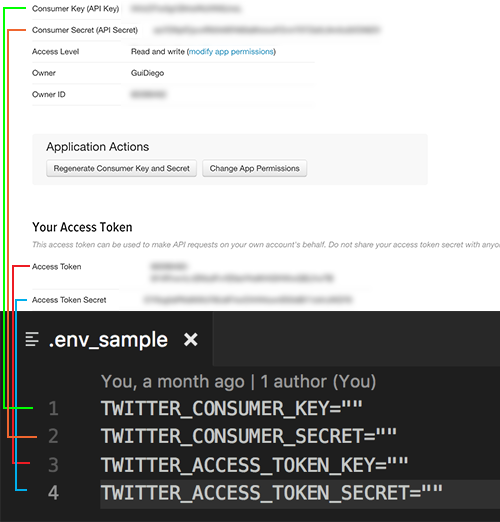
\includegraphics[width=.8\textwidth]{imagens/twitteropts.png}
    \caption{Imagem demonstrando onde cada chave deve ser inserida no código}
    \label{fig:twitteropts}
\end{figure}

Feito isso, é necessário conseguir o JSON de acesso do Google, esse arquivo serve como credencial para que seja possível obter os dados, Figura \ref{fig:twitteropts} pode-se observar que o valor \textit{GOOGLE\_APPLICATION\_CREDENTIALS} já esta definido como \textit{./google\_credentials.json}, ou seja, é necessário apenas baixar as credenciais, move-la para a pastas \textit{dumont/tasks} e renomear para \textit{google\_credentials.json}. Para conseguir acesso a essas credenciais acesse o site da api do Google Language\footnote{\url{https://cloud.google.com/natural-language/}} e clique em \textit{Try it Free}. Feito isso acontecera um redirecionamento para que seja escolhido uma conta google ou, em caso de nenhuma conta estiver previamente autenticada, a tela para efetuar a autenticação. Lembrando que é necessário para quem for replicar a pesquisa ter ao menos uma conta no google (pode ser o mesmo e-mail do gmail). Após selecionado será redirecionado para uma tela informando que o usuário tem 300 dólares gratuitos dentro da google cloud. O primeiro aceite é para receber notificações dos serviços da Google, e pode ficar marcado como "não". O segundo é o aceite dos termos de uso, e esse tem que estar marcado como "sim". Após isso basta clicar em "Agree and Continue". Basta completar algumas informações e informar um cartão de crédito valido (lembrando que isso é apenas um passo de segurança para a google). Feito isso você será direcionado para um \textit{dashboard} da google cloud, como mostrado na figura \ref{fig:googleflow}, basta clicar em \textit{Api \& Services > Credentials}, logo após acessar a tela de credenciais clique em \textit{Create credentials > Service Account Key} após mais um redirecionamento selecione o Serviço (caso não tenha um ainda, basta criar clicando em \textit{New service account}), mantenha a opção JSON marcada e clique em \textit{create}. Logo que fizer isso um JSON com um nome aleatório será baixado em sua máquina, basta mover e renomear como já dito previamente.

\begin{figure}
    \centering
    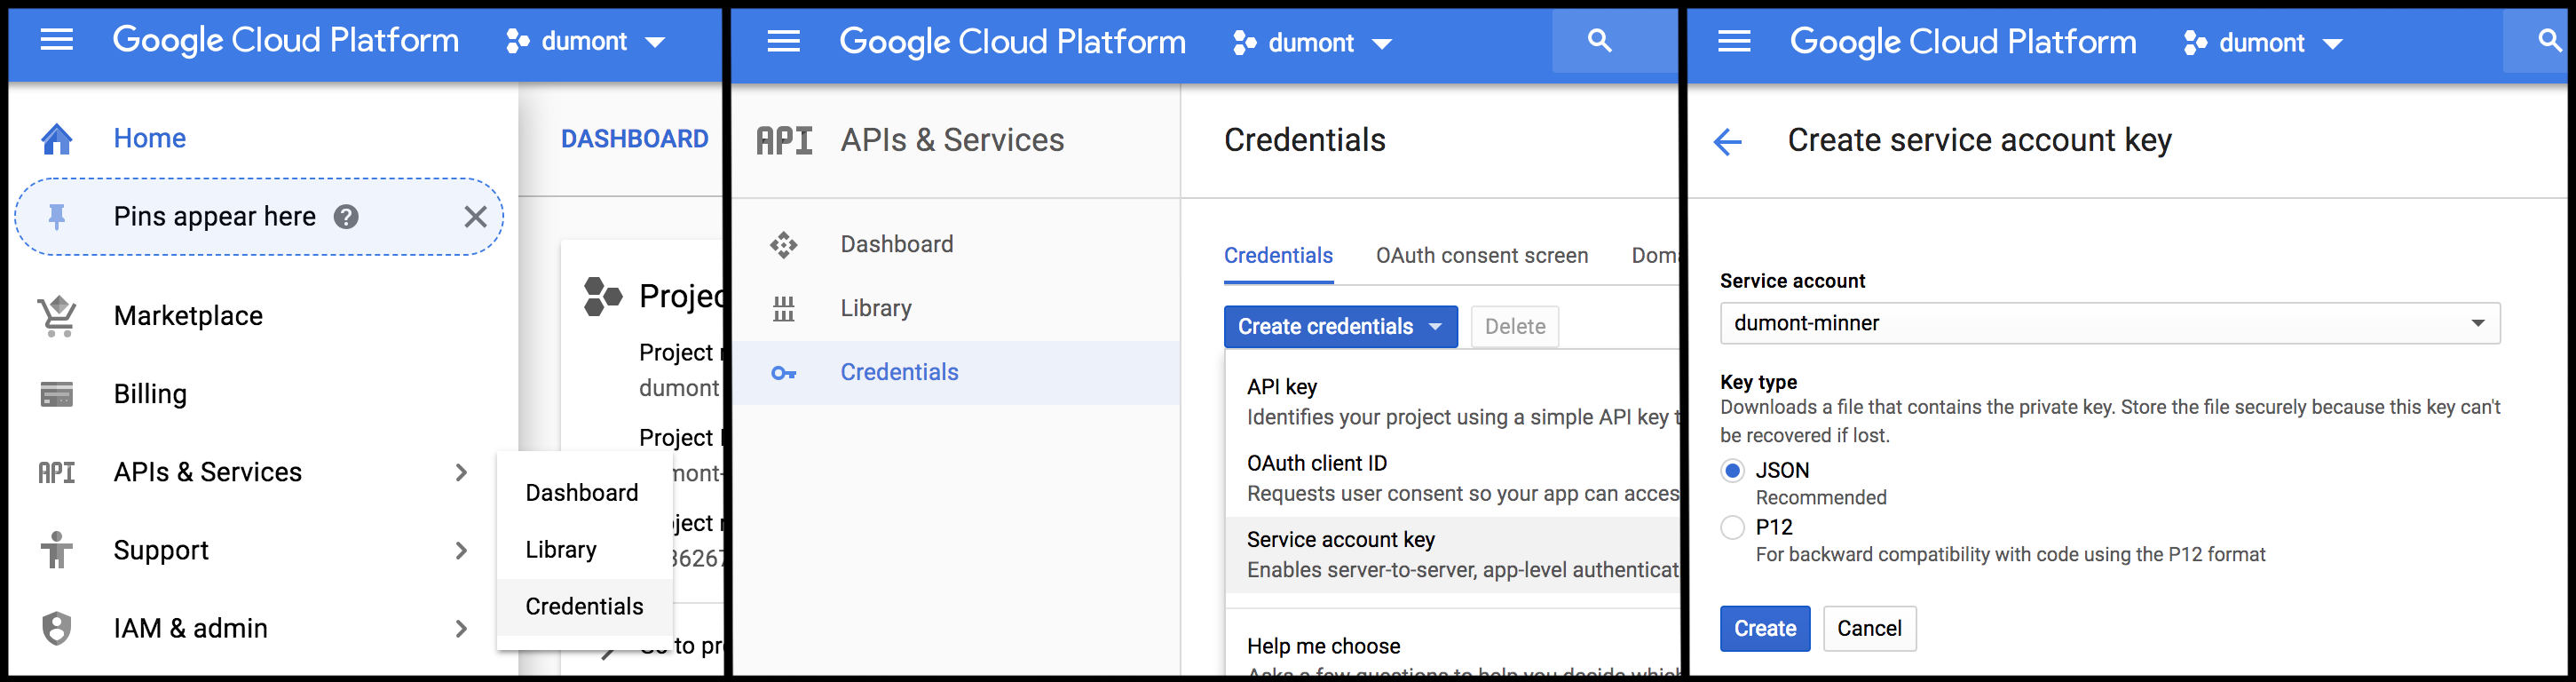
\includegraphics[width=1\textwidth]{imagens/googleflow.png}
    \caption{Imagem demonstrando passo a passo de como gerar o JSON de credencial}
    \label{fig:googleflow}
\end{figure}

Agora é possível executar os comandos, entretanto, existem configurações que devem ser retiradas e/ou alteradas para evitar problemas. Para isso vamos entrar na parte que envolve os processos de coleta e mineração de dados, com o intuito de entender as ultimas configurações e como todo o processo é executado.


\section{Processos}
O trabalho de coleta pode ser dividido em duas grandes partes, a coleta em si e a mineração de dados. Uma parte dessa mineração é feita inteiramente automatizada usando algoritimos e bibliotecas, entretando, existe outra parte que envolve a entrada de dados especialistas.

Nessa sessão séra dado um pequeno detalhamento de como funciona a coleta e a mineração, e como foi utilizado as ferramentas préviamente citadas nesse trabalho. Será iniciado o detalhamento pela coleta, uma vez que é necessário existir algum dado para que seja possível qualquer outra ação


\subsection{Coleta}
Para isso existem ainda algumas configurações pendentes, como podemos observar na figura \ref{fig:creds}, existem duas telas, a primeira é o \textit{dumont/sample\_env} e a segunda a réplica criada anteriormente \textit{dumont/dev.env}, foi removido todas as variáveis referentes aos serviços da AWS, já que não será utilizado local como já abordado, além disso foi retirado o usuário e senha do mongo já que o serviço no docker foi configurado para não precisar do mesmo. Além disso a variável \textit{COLLECTOR\_REQUEST\_TOKEN} pois a intuição dela é criar um mínimo de autenticação caso utilize essa API pública na internet. Por fim o \textit{COLLECTOR\_LIMIT} irá limitar a quantidade de usuarios a serem coletados a cada requisição.

\begin{figure}
    \centering
    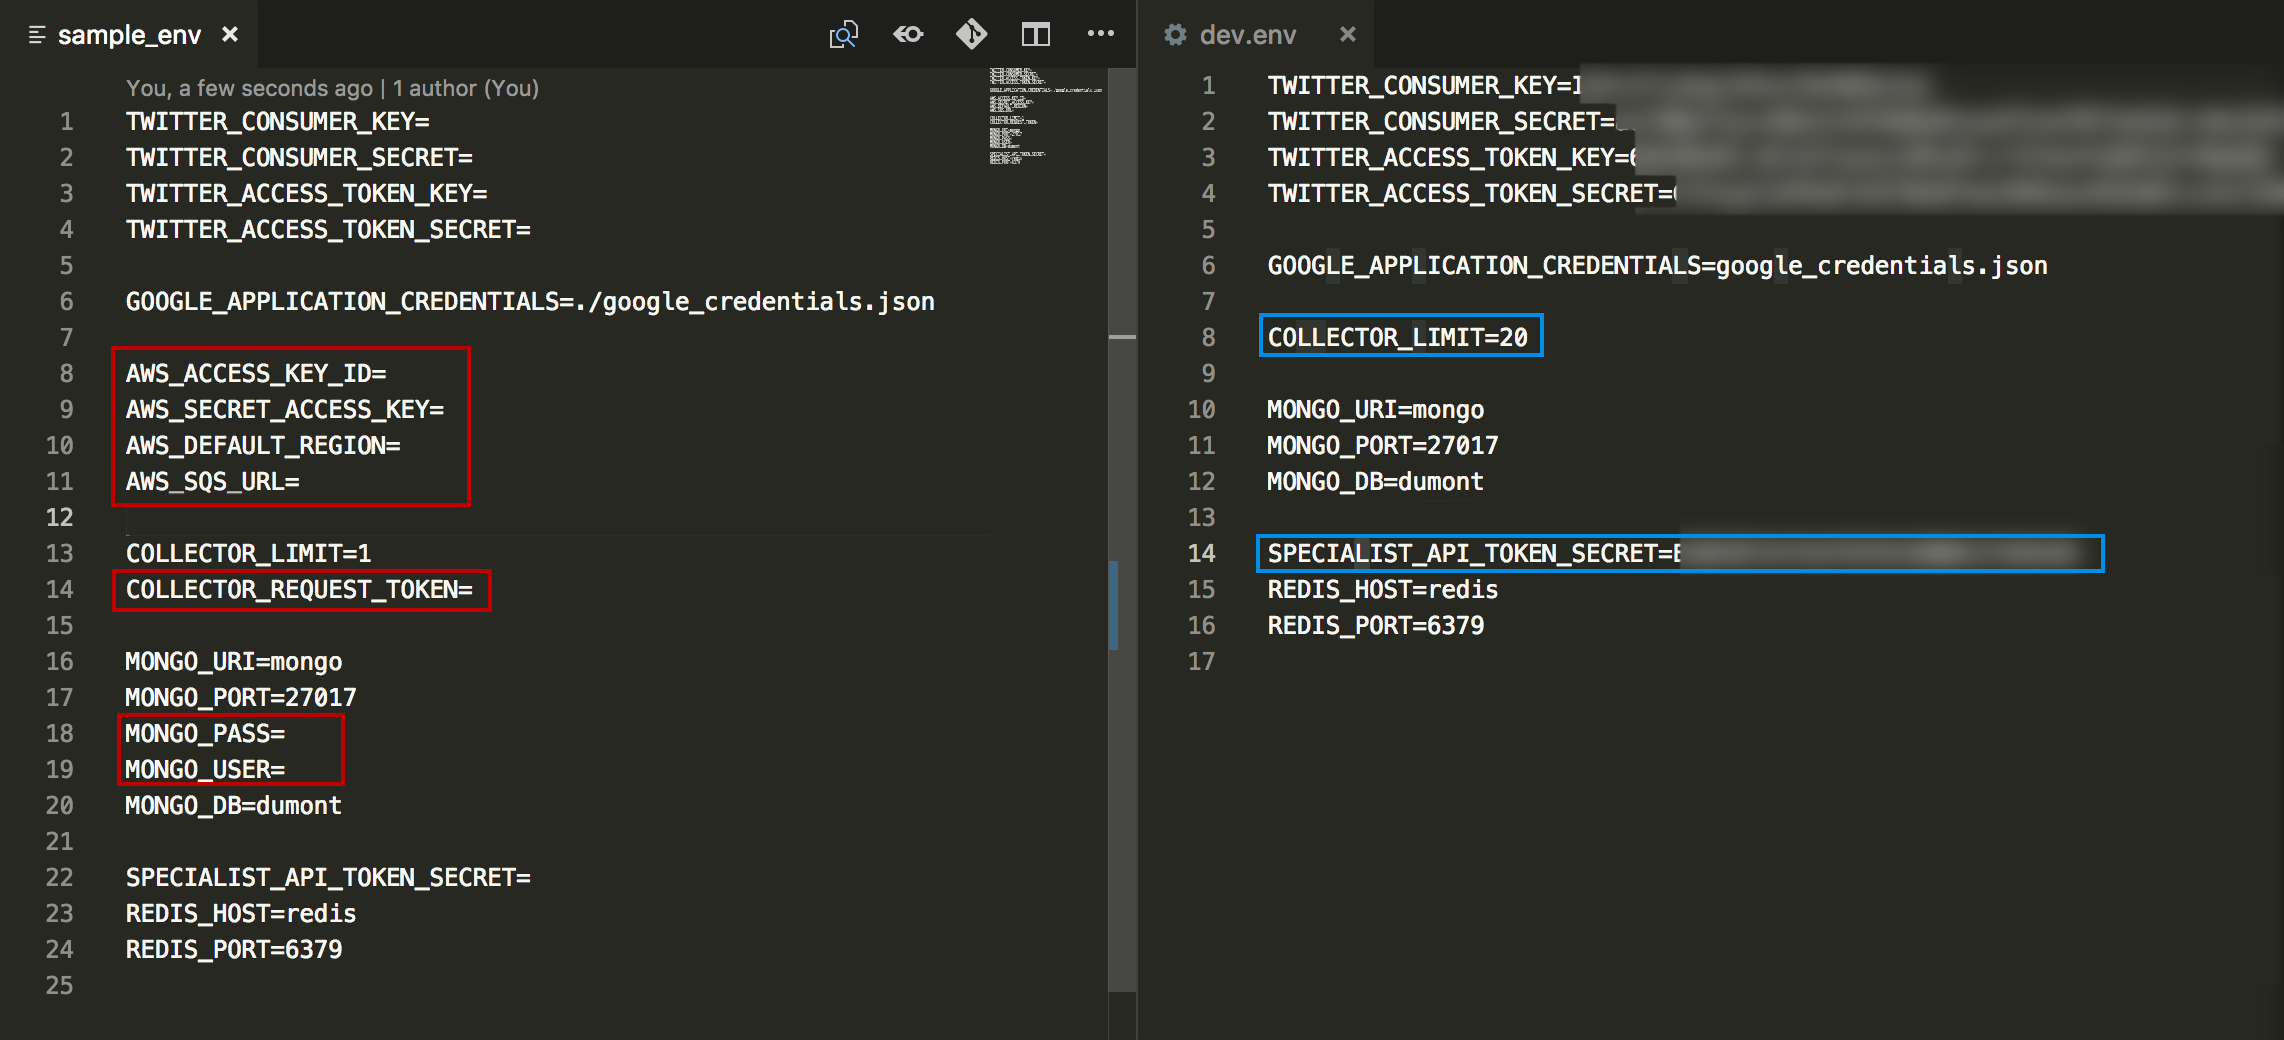
\includegraphics[width=1\textwidth]{imagens/creds.png}
    \caption{Imagem demonstrando passo a passo de como gerar o JSON de credencial}
    \label{fig:creds}
\end{figure}

É importante lembrar dos limites da API publica do twitter, e tambem que devido a implementação (que pode ser acompanhada no arquivo \textit{dumont/collector/twitter/index.js}) na linha 74 é possível ver o momento onde a \textit{stream} é parada, entretando, podem chegar inumeros tweets de diferentes usuarios simuntaneamente, fazendo assim, com que sobrecarregue a quantiadade de usuarios permitidas na API. É sugerido rodar valores baixos entre 20 a 45 para evitar problemas.

Uma vez configurado, é possivel executar o comando \textit{docker-compose -f docker-compose.dev.yml}, uma vez que o docker inicie o serviço você pode iniciar a coleta utilizando desde um navegador, ferramentas (um exemplo é o Postman\footnote{https://www.getpostman.com/}) ou até mesmo o \textit{curl} utilizando o uri \textit{\url{http://127.0.0.1:8080/}}

Depois que os dados foram coletados, ja é possível minerar algumas informações deles, para isso existem processos a serem detalhados.
\subsection{Mineração}
O segundo passo após coletar os dados é rodar scripts de mineração. Uma das maiores dificuldades é como manipular os dados de maneira incremental. Desde que a pesquisa teve inicio, muitas ideias surgiram, novos pontos de vistas e novos dados a serem minerados. Foi adotado uma propriedade chamada \textit{processing_version}, essa propriedade marca o documento com a versão do processamento dele.

Dentro da pasta \textit{dumont/tasks/processing} existe duas pastas, uma para processar usuários e outra para processar tweets, ambas exportam vários estágios de processamento, esse estágio é exportado e passado para uma classe chamada \textit{Processor} localizada no arquivo \textit{dumont/tasks/processing/__init__.py}, o nível de processamento base é o 0 (nível inserido na hora que o coletor salva do dado no banco), a partir disso é possível atualizar o processamento por um script (no caso existe a possibilidade de consumo da fila, porem, como já dito essa abordagem esta contida no anexo 1).

Quando o coletor foi configurado, automaticamente todos os dados necessários para o processamento já foram preenchidos. A tarefa de processamento é responsável por:

\begin{itemize}
    \item Remoção de \textit{stop-words}: Existem palavras que prejudicam a analise textual por não serem essenciais ou estarem colocadas de maneira equivocada. Um dos processos retira esse tipo de ruído do texto.
    \item Arvore Léxica: Criar uma arvore léxica baseada na frase original do tweet e na frase que já foi tratada removendo as \textit{stop-words}.
    \item Analise de Sentimento: Utilizando a API do Google Language é retirado o sentimento da frase original e da frase tratada também.
\end{itemize}

Para obter esses dados basta rodar o comando \textit{docker-compose -f docker-compose.dev.yml up tasks}. Com esses dados já é possível ter alguma noção de informações relevantes dos textos, porém ainda é necessário de embasamento técnico, ou seja, um dado especialista que possa orientar a máquina a utilizar as demais propriedades mapeadas para localizar um delta em comum.

Existe um outros serviços contidos dentro do projeto o \textit{dumont/specialist-api} e \textit{dumont/specialist-app} que gera uma API e uma interface gráfica para injeção de dados especialistas. Para subir ambos os serviços basta utilizar o comando \textit{docker-compose -f docker-compose.dev.yml up specialist-app}. Entretanto, é necessário de um usuário para injetar as analises, é possível criar o documento na mão dentro do mongo, porem, existe um binário dentro da pasta chamado \textit{dumont/create\_specialist}, basta executa-lo passando o e-mail e ele te devolvera uma senha aleatória. Então basta acessar \textit{\url{http://127.0.0.1:3000/}} e utilizar os dados para entrar no sistema. Logo que autenticado você encontrara uma tela igual a da figura \ref{}, nela existe o tweet, uma área para adicionar perguntas da EADS relacionadas, e um local onde pode-se identificar palavras chaves dentro daquele tweet.

Com o sistema rodando, e dados sendo coletados e analisados é necessária uma amostragem para melhor assertividade e desenvolvimento. Durante a pesquisa, em uma preliminar foram coletados mais de 160GB de dados. A amostra foi tirada antes mesmo da inserção de dados especialistas, logo é necessário conhecer os \textit{scripts} de seleção do dumont.

